\documentclass[handout, 10pt]{beamer}

%\usepackage[backend=bibtex,firstinits=true,style=verbose-inote,citestyle=authortitle]{biblatex}
\usepackage{bm}
\usepackage{graphicx}
\usepackage{subcaption}
\usepackage{amsmath}
\usepackage{amsfonts}
\usepackage{makecell}
\usepackage{filecontents}
\usepackage{biblatex}
 \newcommand{\expect}[2][]{
\ifthenelse{\equal{#1}{}}{
\mathbb{E}\left[#2\right]
}{
\underset{#1}{\mathbb{E}}\left[#2\right]
}}

\newcommand{\cov}[2][]{
\ifthenelse{\equal{#1}{}}{
\text{Cov}\left[#2\right]
}{
\underset{#1}{\text{Cov}}\left[#2\right]
}}


\newcommand{\var}[2][]{
\ifthenelse{\equal{#1}{}}{
\text{Var}[#2]
}{
\underset{#1}{\text{Var}}[#2]
}}

\newcommand{\loss}[2][]{
\ifthenelse{\equal{#1}{}}{
\mathcal{L}(#2)
}{
\mathcal{L}_{#1}(#2)
}}

\newcommand{\kl}[2]{
\text{D}_\text{KL}[#1 \parallel #2]
}

\newcommand{\R}{\mathbb{R}}
%\newcommand{\Prob}{\mathbb{P}}

\newcommand{\1}[1]{\mathds{1}\{#1\}}


%\usecolortheme{dolphin}
\setbeamertemplate{navigation symbols}{}
\setbeamertemplate{section in toc}{\inserttocsectionnumber.~\inserttocsection}

\begin{filecontents*}{references.bib}
@InProceedings{GFMN,
author = {Santos, Cicero Nogueira dos and Mroueh, Youssef and Padhi, Inkit and Dognin, Pierre},
title = {Learning Implicit Generative Models by Matching Perceptual Features},
booktitle = {The IEEE International Conference on Computer Vision (ICCV)},
month = {October},
year = {2019}
}
\end{filecontents*}

\addbibresource{references.bib}


\title{Learning Implicit Generative Models by Matching Perceptual Features\footnote{\citepaper{GFMN}}}
%\subtitle{}
%\author{Ivan Skorokhodov}
%\date{}
%\logo{
\includegraphics[height=1cm]{images/ipavlov-logo.png}}

\newcommand{\citepaper}[1]{\citetitle{#1} by \citeauthor{#1}}

%\graphicspath{{./images}}

%\usetheme{lucid}
\begin{document}

\begin{frame}
    \titlepage
\end{frame}

\begin{frame}{Overview}
    \begin{itemize}
        \item\pause Authors train a ``non-standard'' generative model by matching perceptual features:
        \begin{enumerate}
            \item\pause Define a generator $G(z)$ with $z \sim \mathcal{N}(0, I)$
            \item\pause Take an ImageNet-pretrained classifier $E(x)$
            \item\pause Compute data mean $\mu_\text{data}$ and covariance $\Sigma_\text{data}$
            \item\pause Optimize $G(z)$ in such a way that generated mean and covariance is close to real ones
        \end{enumerate}
        \item\pause They propose ADAM moving average of the moments to make the statistics more robust
        \item\pause They perform some theoretical exploration of the approach
        \item\pause Their model achieves quite good results on CIFAR-10 and STL-10
    \end{itemize}
\end{frame}

%\begin{frame}{Inception Score (IS)}
%    \begin{enumerate}
%        \item\pause Take Inception classifier
%        \item\pause Generate a lot of samples
%        \item\pause For each sample $x$ compute class probabilities $p(y|x)$
%        \item\pause Average them to approximately compute $p(y) \approx \expect[p_g(x)]{p(y|x)}$
%        \item\pause Compute \textit{inception score}:
%\begin{equation}
%\mathrm{IS}=\exp \left(\expect[p_{g}(x)]{D_{K L}(p(y | x)|| p(y))}\right)
%\end{equation}
%    \end{enumerate}
%
%\pause
%Intuition:
%\begin{itemize}
%    \item\pause If samples represent meaningful objects then $p(y|x)$ is one-hot
%    \item\pause If samples are diverse then $p(y)$ is uniform
%    \item\pause This gives very high values for KL between $p(y|x)$ and $p(y)$.
%\end{itemize}
%
%\end{frame}
%
%\begin{frame}{Frechet Inception Distance (FID)}
%    \begin{enumerate}
%        \item\pause Take feature extractor from Inception classifier
%        \item\pause Generate a lot of samples and:
%            \begin{enumerate}
%                \item\pause Compute embeddings for them
%                \item\pause Compute statistics $\mu_g, \Sigma_g$ for embeddings
%            \end{enumerate}
%        \item\pause Take a lot of real images and:
%            \begin{enumerate}
%                \item\pause Compute embeddings for them
%                \item\pause Compute statistics $\mu_r, \Sigma_r$ for embeddings
%            \end{enumerate}
%        \item\pause Compute Frechet distance between two Guassians:
%\begin{equation}
%\mathrm{FID}=\left\|\mu_{r}-\mu_{g}\right\|^{2}+\operatorname{Tr}\left(\Sigma_{r}+\Sigma_{g}-2\left(\Sigma_{r} \Sigma_{g}\right)^{1 / 2}\right)
%\end{equation}
%\end{enumerate}
%
%\pause
%Intuition:
%\begin{itemize}
%    \item\pause We directly measure the distribution
%    \item\pause It is not obvious why we do that with FD instead of KL/JS/etc
%\end{itemize}
%    
%\end{frame}


\begin{frame}{Maximum Mean Discrepancy (informally)}
\begin{itemize}
    \item \pause Imagine, that we have a kernel function $k(x, x)$ for $x \in \mathcal{X}$. We define \textit{Reproducing Kernel Hilbert Space (RKHS)} $\mathcal{H}_k$: a set of all real-valued functions on $\mathcal{X}$ (considering that $\mathcal{X}$ is a ``good'' space).
    \item\pause $\mathcal{H}_k$ can have an inner product, for example:
\begin{equation*}
    \langle f, g\rangle_{\mathcal{H}_k} = \int_X f(x) \overline{g(x)} d\mu(x)
\end{equation*}

\item\pause This allows us to compute norms and distances between functions.

\item \pause \textit{Maximum Mean Discrepancy (MMD)} is defined between 2 probability distributions $p$ and $q$ as:
\begin{equation*}
\text{MMD}_k(p, q) = \| \mu_p - \mu_q \|_{\mathcal{H}_k},
\end{equation*}
where $\mu_p = \expect[p(x)]{k_x(.)}$ is the expectation of functions $k_x(.) = k(x, .)$.
\end{itemize}
\end{frame}

\begin{frame}{MMD and generative modeling}
\begin{itemize}
    \item\pause If the kernel $k(x,x)$ is \textit{universal} (approximates functions well), then $\text{MMD}_k(p,q) = 0$ iff $p = q$.
    \item\pause In theory, this gives us a way to build a generative model: just minimize $\text{MMD}_k(p_\text{data}, q_\theta)$ where $q_\theta$ is your neural network
    \item\pause In practice, this gives us nothing: $\mu_p$ and $\mu_q$ are infinite-dimensional so there is no practical way we can optimize them directly.
    \item\pause Luckily, we can rewrite $\text{MMD}$ using the kernel:
\begin{equation*}
\begin{aligned}
\left\|\mu_{p}-\mu_{q}\right\|_{\mathcal{H}}^{2}=&\left\langle\mu_{p}-\mu_{q}, \mu_{p}-\mu_{q}\right\rangle \\
=& \expect[p, p]{\langle k_x, k_{x^\prime}\rangle}
-2 \expect[p, q]{\langle k_x, k_y\rangle}
+\expect[q,q]{\langle k_y, k_{y^\prime}\rangle} \\
=& \expect[p, p]{k(x, x^{\prime})} - 2 \expect[p, q]{k(x, y)} +\expect[q, q]{k(y, y^{\prime})}
\end{aligned}
\end{equation*}
\item\pause But this is not a way authors build their model
\end{itemize}
\end{frame}

\begin{frame}{MMD and feature maps}
\begin{itemize}
    \item\pause One can define a kernel by using \textit{feature maps}: some functions $\phi_j: \mathcal{X} \to \mathbb{R}$ which takes an image $x$ and produce some scalar
    \item\pause Several feature maps $\phi_1, ..., \phi_n, ...$ give us embedding $\Phi(x)$
    \item\pause Now we define kernel $K_\phi(x,y) = \langle \Phi(x), \Phi(y) \rangle$
    \item\pause If the set of feature maps is universal (approximates any function well), then the resulted kernel is universal as well.
    \item\pause ImageNet-pretrained encoder $E$ which outputs an embedding of size $512$ can be seen as a set of 512 individual feature maps $\phi_1, ..., \phi_{512}$
    \item\pause And it gives us a way to minimize $\text{MMD}_{K_\Phi}(p_\text{data}, q_\theta)$ with:
\[
\langle \Phi(x), \Phi(y) \rangle = \Phi(x)^\top \Phi(y)
\]
    \item\pause These feature maps must be kept fixed during optimization
    \item\pause As far as I understand, feature maps for a neural network cannot be universal...
%    \item\pause Some smart people brought \textit{feature maps} to the kernel theory --- functions that embed your objects in a feature space.
%    \item\pause Now you can embed object $x$ with $\phi(.)$ before applying a kernel $k$.
%    \item\pause This gives us a new kernel $K_\phi(x, y) = k(\phi(x), \phi(y))$
\end{itemize}
\end{frame}

\begin{frame}{Generative Feature Matching Network (GFMN)}
\begin{itemize}
    \item\pause Authors propose to optimize MMD using ImageNet-pretrained encoder as a feature embedder $\Phi(x)$.
    \item\pause In this case MMD is formulated as:
\begin{equation}
\mathrm{MMD}^{2}_{K_{\Phi}}(p, q)=\|\expect[x \sim p]{\Phi(x)} - \expect[x \sim q]{\Phi(x)}\|^2
\end{equation}
    \item\pause Which is basically matching mean features between real and fake distributions:
\begin{figure}
    \centering
    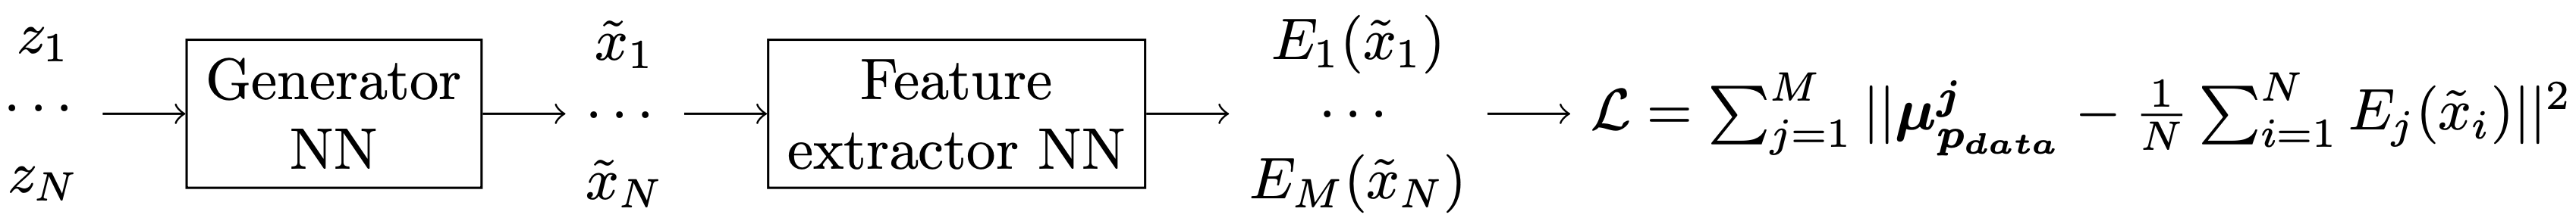
\includegraphics[width=0.9\textwidth]{images/gfmn-scheme}
\end{figure}
    \item\pause To theoretically justify matching covariances one need to introduce new feature maps of the kind $\phi_i(x) \phi_j(x)$
\end{itemize}
\end{frame}


\begin{frame}{GFMN: what happens in practice}
\pause
In practice, authors optimize the following loss:
\begin{equation}
\min _{\theta} \sum_{j=1}^{M}\left\|\mu_{p_{\text {data }}}^{j}-\mu_{p_{G}}^{j}(\theta)\right\|^{2}+\left\|\sigma_{p_{\text {data }}}^{j}-\sigma_{p_{G}}^{j}(\theta)\right\|^{2},
\end{equation}
where $M$ is the number of layers we gather the features from.

\pause
Here $\sigma$ is a diagonal covariance since matching full covariances is too expensive:
\begin{equation}
\begin{aligned}
\sigma_{p_{\text {data}}, \ell}^{j} &=\expect[x \sim p_{\text{data}}]{E_{j, \ell}(x)^{2}} - \left(\mu_{p_{\text {data}}}^{j, \ell}\right)^{2}, \ell=1 \ldots d_{j} \\
\sigma_{p_{G}, \ell}^{j}(\theta) &= \expect[z]{E_{j, \ell}(G(z ; \theta))^{2}}-\left(\mu_{p_{G}}^{j, \ell}\right)^{2}, \ell=1 \ldots d_{j}
\end{aligned}
\end{equation}
\end{frame}


\begin{frame}{ADAM Moving Average (AMA)}
\begin{itemize}
    \item\pause We can rewrite MMD for means as:
    \[
    \|\mu_p - \mu_q\|^2 = (\mu_p - \mu_q)^\top (\mu_p - \mu_q) = \Delta^\top (\mu_p - \mu_q)
    \]
    \item\pause Where $\mu_q = \expect[z]{E(G(z)}$, and we can approximate it on a minibatch of size $N$: $\hat\mu_q = \frac{1}{N}\sum_i E(G(z_i))$
    \item\pause To make the estimate more robust authors propose to use a moving average of $\Delta$:
    \[
    \|\mu_p - \mu_q\|^2 \approx v^\top (\mu_p - \mu_q)
    \]
    where $v$ is a moving average of $\Delta$:
    \[
    v_\text{new} = (1 - \alpha) v_\text{old} + \alpha \Delta
    \]
    \item\pause This formula is equivalent to a gradient step towards minimizing
    \[
L(v) = \frac{1}{2}\left\|v-\Delta_{j}\right\|^{2}
    \]
    \item\pause Authors propose to update $v$ by minimizing $L(v)$ with Adam optimizer.
\end{itemize}
\end{frame}

\begin{frame}{Using AMA turend out to be very important}
Apparently, even batch size of 512 is not enough to compute a good estimate:
\begin{figure}
\centering
\includegraphics[width=\textwidth]{images/gfmn-ama.png}
\end{figure}
\end{frame}

\begin{frame}{Results}
\begin{figure}
\centering
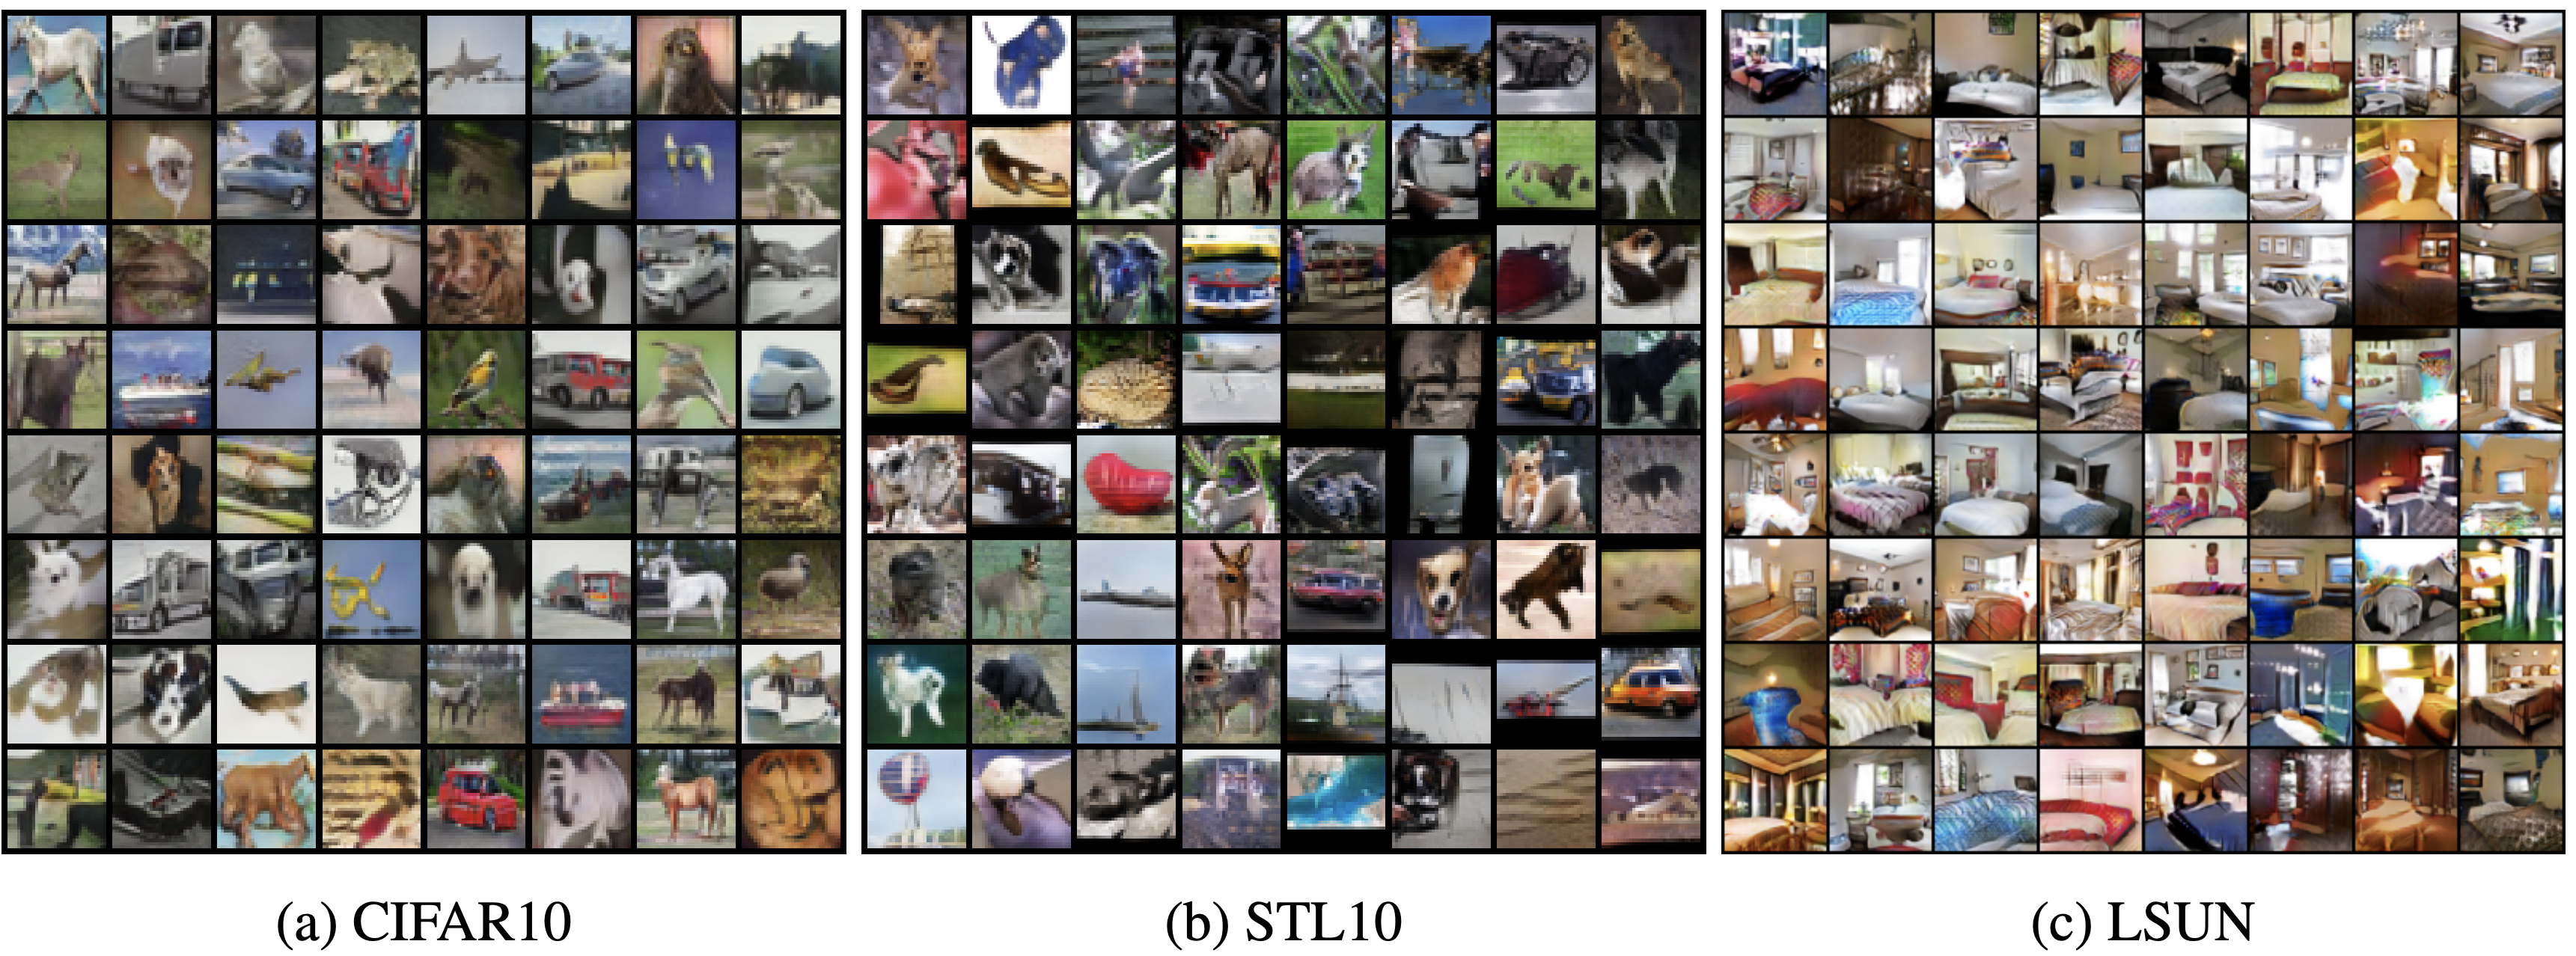
\includegraphics[width=\textwidth]{images/gfmn-samples.png}
\end{figure}
\end{frame}

\begin{frame}{Loss function value is correlated well with sample quality}
\begin{figure}
\centering
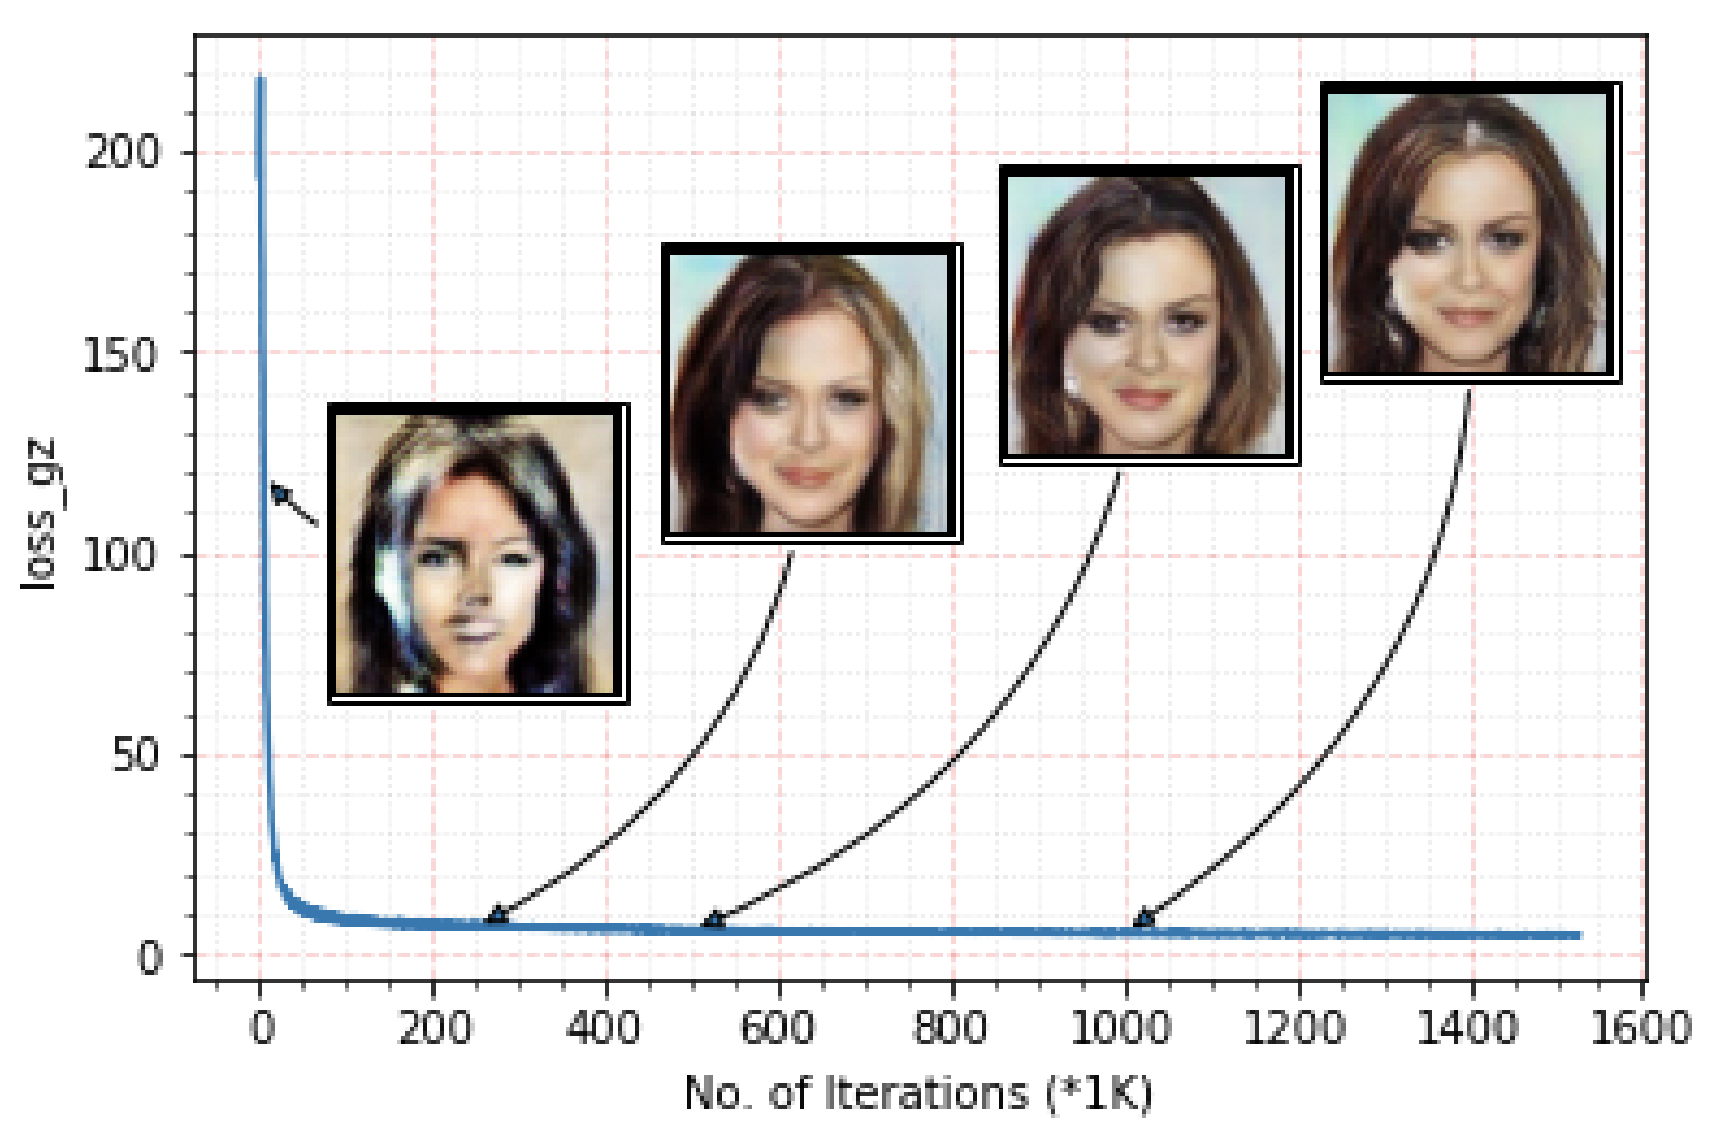
\includegraphics[width=0.8\textwidth]{images/gfmn-loss-plot.png}
\end{figure}
\end{frame}

\begin{frame}{Quantitive results}
\begin{figure}
\centering
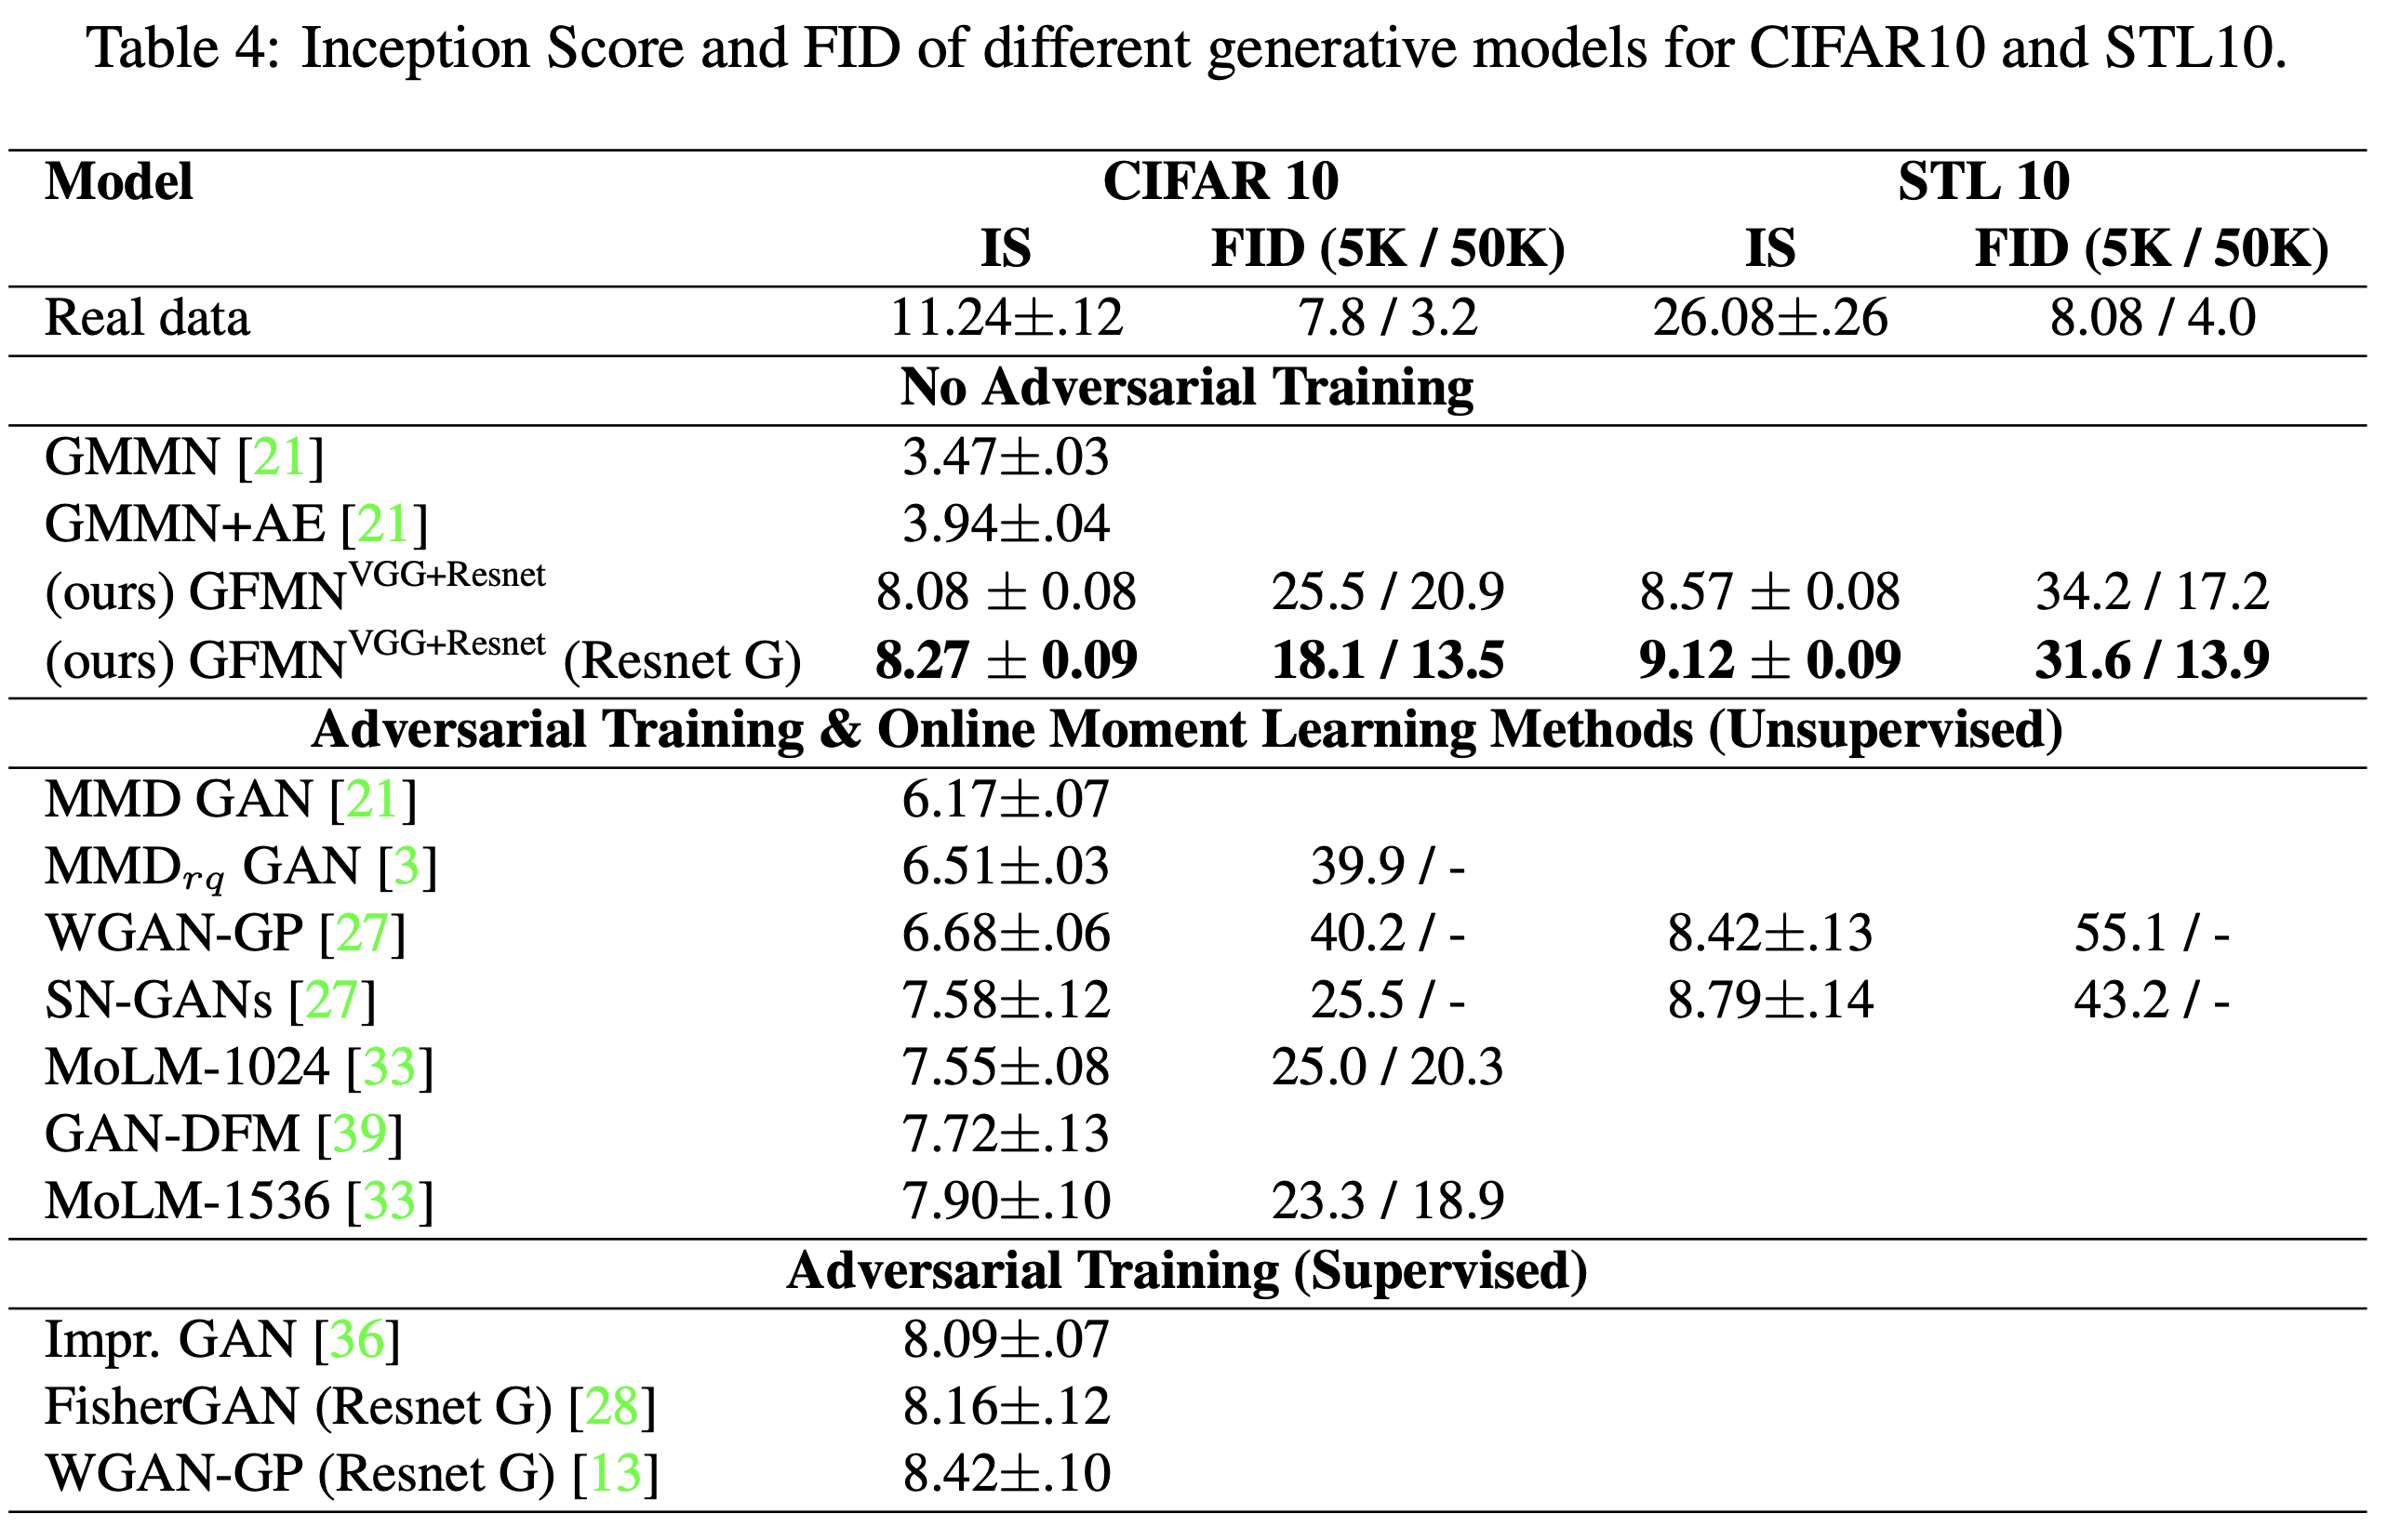
\includegraphics[width=0.8\textwidth]{images/gfmn-results.png}
\end{figure}
\end{frame}


\begin{frame}{Conclusion}
\begin{itemize}
    \item Benefit 1: the loss function is directly correlated with the generated image quality
    \item Benefit 2: no mode collapse
    \item Benefit 3: one can use several encoders to improve scores and this encoders are cross-domain
    \item In some way their objective is quite close to FID, so in some sense they optimize a final evaluation metric directly
\end{itemize}
\end{frame}


\end{document}
